\documentclass[twocolumn]{extarticle}
\usepackage{fontspec}   %加這個就可以設定字體
\usepackage{xeCJK}       %讓中英文字體分開設置
\usepackage{indentfirst}
\usepackage{listings}
\usepackage[newfloat]{minted}
\usepackage{float}
\usepackage{graphicx}
\usepackage{caption}
\usepackage{fancyhdr}
\usepackage{hyperref}
\usepackage{amsmath}
\usepackage{multirow}
\usepackage[dvipsnames]{xcolor}
\usepackage{graphicx}
\usepackage{tabularx}
\usepackage{booktabs}
\usepackage{caption}
\usepackage{subcaption}
\usepackage{pifont}
\usepackage{amssymb}
\usepackage{titling}
\usepackage{physics}



\usepackage{pdftexcmds}
\usepackage{catchfile}
\usepackage{ifluatex}
\usepackage{ifplatform}

\usepackage[breakable, listings, skins, minted]{tcolorbox}
\usepackage{etoolbox}
\setminted{fontsize=\footnotesize}
\renewtcblisting{minted}{%
    listing engine=minted,
    minted language=python,
    listing only,
    breakable,
    enhanced,
    minted options = {
        linenos, 
        breaklines=true, 
        breakbefore=., 
        % fontsize=\footnotesize, 
        numbersep=2mm
    },
    overlay={%
        \begin{tcbclipinterior}
            \fill[gray!25] (frame.south west) rectangle ([xshift=4mm]frame.north west);
        \end{tcbclipinterior}
    }   
}

\usepackage[
top=1.5cm,
bottom=0.75cm,
left=1.5cm,
right=1.5cm,
includehead,includefoot,
heightrounded, % to avoid spurious underfull messages
]{geometry} 

\newenvironment{code}{\captionsetup{type=listing}}{}
\SetupFloatingEnvironment{listing}{name=Code}
\usepackage[moderate]{savetrees}


\title{NYCU Introduction to Machine Learning, Homework 3}
\author{110550088 李杰穎}
\date{}


\setCJKmainfont{Noto Serif TC}


\ifwindows
\setmonofont[Mapping=tex-text]{Consolas}
\fi

\XeTeXlinebreaklocale "zh"             %這兩行一定要加,中文才能自動換行
\XeTeXlinebreakskip = 0pt plus 1pt     %這兩行一定要加,中文才能自動換行

\setlength{\parindent}{0em}
\setlength{\parskip}{2em}
\renewcommand{\baselinestretch}{1.25}
\setlength{\droptitle}{-7.5em}   % This is your set screw
\setlength{\columnsep}{2em}
\usepackage{enumitem}

\begin{document}

\maketitle

\section{Part. 1, Coding}
\subsection{Decision Tree}
\begin{enumerate}
\item Compute the gini index and the entropy of the array [0, 1, 0, 0, 0, 0, 1, 1, 0, 0, 1].

\autoref{fig:decisiontreeres} shows the results of gini index and the entropy of given array.

\item Show the accuracy score of the testing data using \texttt{criterion='gini'} and \texttt{max\_depth=7}. Your accuracy score should be higher than 0.7.

\autoref{fig:decisiontreeres} shows the accuracy score of testing data using \texttt{criterion='gini'} and \texttt{max\_depth=7}. The accuracy score is 0.705.

\item Show the accuracy score of the testing data using \texttt{criterion='entropy'} and \texttt{max\_depth=7}. Your accuracy score should be higher than 0.7.

\autoref{fig:decisiontreeres} shows the accuracy score of the testing data using \texttt{criterion='entropy'} and \texttt{max\_depth=7}. The accuracy score is 0.721.

\item Train your model using \texttt{criterion='gini', max\_depth=15}. Plot the feature importance of your decision tree model by simply counting the number of times each feature is used to split the data. 

\autoref{fig:featureimportance} is the plot of feature importance of decision tree with \texttt{criterion='gini', max\_depth=15}.

\end{enumerate}

\begin{figure}[H]
\centering
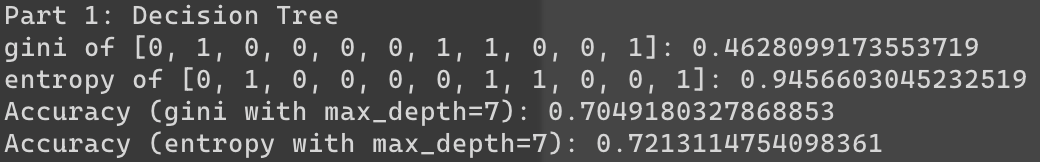
\includegraphics[width=0.95\linewidth]{decision_tree_res}
\caption{The gini index and entropy of given array and the accuracy of decision tree using these two criterions with maximum depth is 7.}
\label{fig:decisiontreeres}
\end{figure}

\begin{figure}[H]
\centering
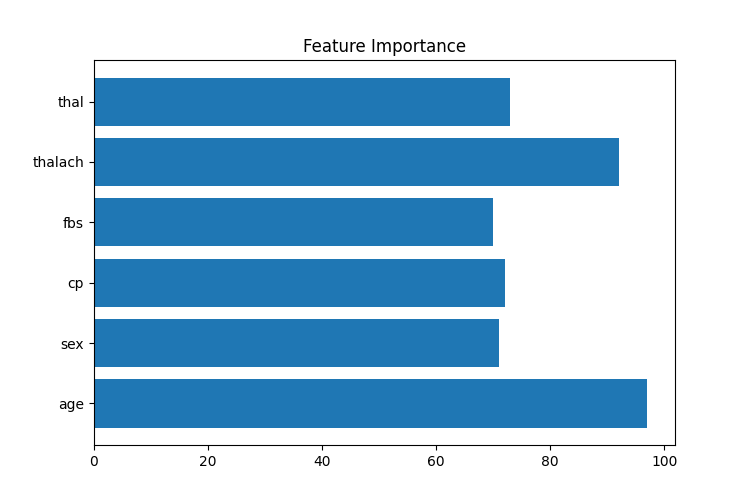
\includegraphics[width=0.95\linewidth]{feature_importance}
\caption{The plot of feature importance of decision tree with \texttt{max\_depth=15, criterion='gini'}.}
\label{fig:featureimportance}
\end{figure}




\subsection{Adaboost}

\begin{enumerate}
\setcounter{enumi}{4}
\item Tune the arguments of AdaBoost to achieve higher accuracy than your Decision Trees.

As in \autoref{fig:adaboostres}, the accuracy score is 0.82, which is higher than decision tree. This is achieved by \texttt{random\_seed=156, n\_estimators=20}.
\end{enumerate}

\begin{figure}[H]
\centering
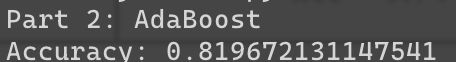
\includegraphics[width=0.95\linewidth]{adaboost_res}
\caption{The accuracy score of Adaboost algorithm}
\label{fig:adaboostres}
\end{figure}


\section{Part. 2, Questions}

\begin{enumerate}
	\item True or False
	\begin{enumerate}[label=\alph*.]
		\item In an iteration of AdaBoost, the weights of misclassified examples are increased by adding the same additive factor to emphasize their importance in subsequent iterations.
		
		False. First, the weights of misclassified example are updated by multiplying by some factor, not by adding. Second, the weights of misclassified example are not always increased, because when weak classifier is too weak (i.e. accuracy is below 0.5), the $\alpha$ will be less than 0. Leading to decreasing of weights of misclassified example.
		
		\item AdaBoost can use various classification methods as its weak classifiers, such as linear classifiers, decision trees, etc.
		
		True.
	\end{enumerate}
	\item How does the number of weak classifiers in AdaBoost influence the model's performance? Please discuss the potential impact on overfitting, underfitting, computational cost, memory for saving the model, and other relevant factors when the number of weak classifiers is too small or too large.
	
	\begin{itemize}
	\item \textbf{Overfitting and Underfitting}: If the number of weak classifiers is too small, the adaboost model may underfit. Underfitting occurs when the model is too simple to capture the complexities and patterns in the data, leading to poor performance. In the contrast, if the number of weak classifiers is too large, the model may overfit. Overfitting happens when the model becomes too complex, capturing not only the underlying patterns but also the noise in the training data. This leads to high accuracy on the training dataset but poor generalization to new, unseen data.
	\item \textbf{Computational Cost}: The model is quicker to train and inference when the number of weak classifier is small. This is can be advantageous when the computation resources is limited. Conversely, when there has too many weak classifiers, the model takes longer time to train because it involves more iterations. This can be a significant disadvantages when training on a larger dataset.
	\item \textbf{Memory for Saving the Model}: If the number of weak classifier is small, then we don't need lots of memory to store the model. However, if the number of weak classifier is large, it will require more memory to store all these classifiers. This can be a limitation when deployed the model in a memory-constrained environment.
	\item \textbf{Other Relevant Factors}: The first one is interpretability, model with fewer weak classifier is tends to be easier to interpret and understand. As the complexity of the model increased along with the number of weak classifiers. The second one is generalizability, while a certain number of weak classifiers are necessary for the model to capture the complexity of the data, beyond a certain point, adding more classifiers might not significantly improve the model's ability to generalize to new data. 
	\end{itemize}
	
	\item A student claims to have a brilliant idea to make random forests more powerful: since random forests prefer trees which are diverse, i.e., not strongly correlated, the student proposes setting $m = 1$, where $m$ is the number of random features used in each node of each decision tree. The student claims that this will improve accuracy while reducing variance. Do you agree with the student's claims? Clearly explain your answer.
	
	First, increasing diversity among trees in a Random Forest is indeed beneficial. It helps in reducing the correlation between individual trees, which in turn reduces the variance of the overall model. However, diversity must be balanced with the individual strength of each tree. If each tree becomes too weak (poor at predicting), the overall performance of the forest can suffer.
	
	Normally, $m$ will set to a number between 1 and the number of features. By setting $m=1$, each split in each tree would consider only one randomly selected feature. This approach would indeed increase the diversity among the trees, as each tree would be making decisions based on a very different set of features. However, this extreme randomness can lead to each tree being very weak, particularly if the dataset has a large number of features where only a few are strongly predictive. In such cases, the chance of selecting the most informative feature at each split becomes very low.
	
	In summary, setting $m=1$ is a extreme version of random forests. While it maximizes the diversity, it likely to make the individual trees weaker, especially in datasets where features relevance varies significantly. Practically, the $m$ should be treated as hyperparameter, and should be tuned based on the characteristic of datasets. Directly set $m=1$ may not always a good idea. 
	
	
	\item The formula on the left is the forward process of a standard neural network while the formula on the right is the forward process of a modified model with a specific technique.
	\begin{figure}[H]
	\centering
	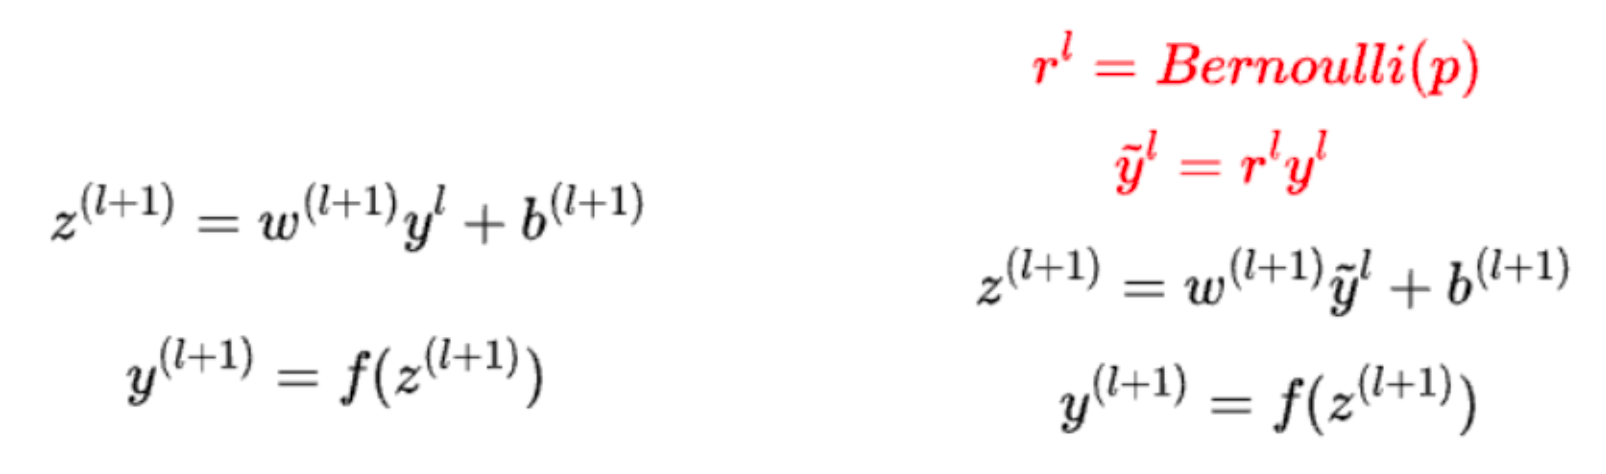
\includegraphics[width=0.95\linewidth]{report_q}
	\caption{}
	\label{fig:reportq}
	\end{figure}
	
	\begin{enumerate}[label=\alph*.]
		\item According to the two formulas, describe what is the main difference between the two models and what is the technique applied to the model on the right side.
		
		The main difference between two models is the introduction of the $r^l$ term on the right, which comes from a Bernoulli distribution with parameter $p$. The Bernoulli distribution is a distribution that output 1 with probability $p$. By introducing this term, the model will randomly drop units (i.e. set to zero the output of some neurons) during training, which is a technique known as dropout. Dropout helps prevent overfitting by forcing the network to learn more robust features that are not reliant on any single subset of the neurons.
		
		\item This technique was used to deal with overfitting and has many different explanations; according to what you learned from the lecture, try to explain it with respect to the ensemble method.
		
		Dropout can be interpreted as a form of model averaging, which is an ensemble technique. During training, each mini-batch effectively trains a different "thinned" network (a network with some units dropped out), and at test time, it's like averaging the outputs of these many thinned networks. This is similar to creating an ensemble of different models, where each model is trained on a different subset of the data or features, and then the predictions of all models are averaged to obtain the final output. Dropout harnesses the power of ensemble learning within a single model architecture by using stochasticity during training.
	\end{enumerate}
\end{enumerate}



\end{document}

 